\chapter{Implementation and benchmarks}

Both algorithms are implemented in \texttt{C++20} as a contribution to an open-source library \texttt{Koala NetworKit} \cite{koala_networkit}. In order to implement these algorithms, we used three helper libraries: \texttt{NetworKit} \cite{networkit}, \texttt{Eigen} \cite{eigen} and \texttt{NTL} \cite{ntl}. The first one provides a graph class, as well as some graph related utility functions. Because of the algebraic nature of the presented algorithms, we also decided to include the \texttt{Eigen} and the \texttt{NTL} library.

\section{Gaussian matching}
\subsection{Implementation details}
We expanded on the pseudocode provided by Mucha and Sankowski in \cite{mucha} to create a implementation of the Gaussian matching algorithm. The key part of the implementation is included in five files:
\begin{itemize}
    \item \texttt{GeneralGaussianMatching.cpp} and \texttt{NaiveGaussianMatching.cpp}*
    \item \texttt{BipartiteGaussianMatching.cpp}
    \item \texttt{LazyGaussElimination.cpp} and \texttt{NaiveGaussElimination.cpp}*
    \item \texttt{NaiveDynamicComponents.cpp}*
\end{itemize}

The first two files represent the algorithm from \cite{mucha}. The first one is capable of solving a bipartite case of the problem, while the second one computes a perfect matching for the general graphs. One of our contributions is the \textsc{GaussEliminationAlgorithm}. We developed both a naive version as well as a optimal \textsc{LazyGaussElimination} that runs in $O(n^\omega)$ time. The second version was only described in the original work of Mucha \cite{mucha}. Based on the description we developed a pseudocode and a working \texttt{C++} code.
The last file represents a data structure that has only a naive implementation. Providing an implementation based on \cite{dynamic_components} will be likely to further improve the running time of the algorithm. 

We first tried to use \texttt{Eigen} \cite{eigen} for all matrix computations. It however turned out to be insufficient to handle finite field operations. Abandoning $Z_p$ field for a floating point matrices introduced some issues to the implementation. Both the values of cells in the skew matrix and the determinant of the matrix itself can not be to small or to big. This would lead to a precision issues when working with a floating point data types. To avoid this issue we decided to use a number theory focused library - \texttt{NTL} \cite{ntl}.

\subsection{Benchmark}
We present a benchmark comparing the running time of the implemented algorithms. For the additional context, we compare the result to some of the maximum matching algorithms already implemented in \texttt{Koala/NetworKit}. The algorithms were tested on two separate categories. The first chart regard a bipartite graphs, while the second one represents a general case. Here we present an average runtime of the algorithms, averaged over $10$ different random graphs. Each graph has exactly $n$ vertices and $m$ edges. In addition, each graph has a perfect matching.

\begin{table}[H]
\centering
\label{tab:benchmark}
\begin{tabular}{lccc}
\hline
\textbf{Algorithm} 
& \begin{tabular}[c]{@{}c@{}}$n=100$ \\ $m=2000$\end{tabular}
& \begin{tabular}[c]{@{}c@{}}$n=1000$ \\ $m=200000$\end{tabular} \\
\hline
\textsc{NaiveGaussianMatching} & 129 ms & 129.67 s \\
\textsc{GeneralGaussianMatching} & 66 ms & 4.96 s \\
\textsc{BipartitegGaussianMatching} & 7 ms & 4.88 s \\
\hdashline
\textsc{EdmondsMaximumMatching} & 2 ms & 2.35 s \\
\textsc{GabowMaximumMatching} & 3 ms & 3.35 s \\
\hline
\end{tabular}
\caption{Benchmark Results for Bipartite Graph Matching}
\end{table}

\begin{figure}
\centering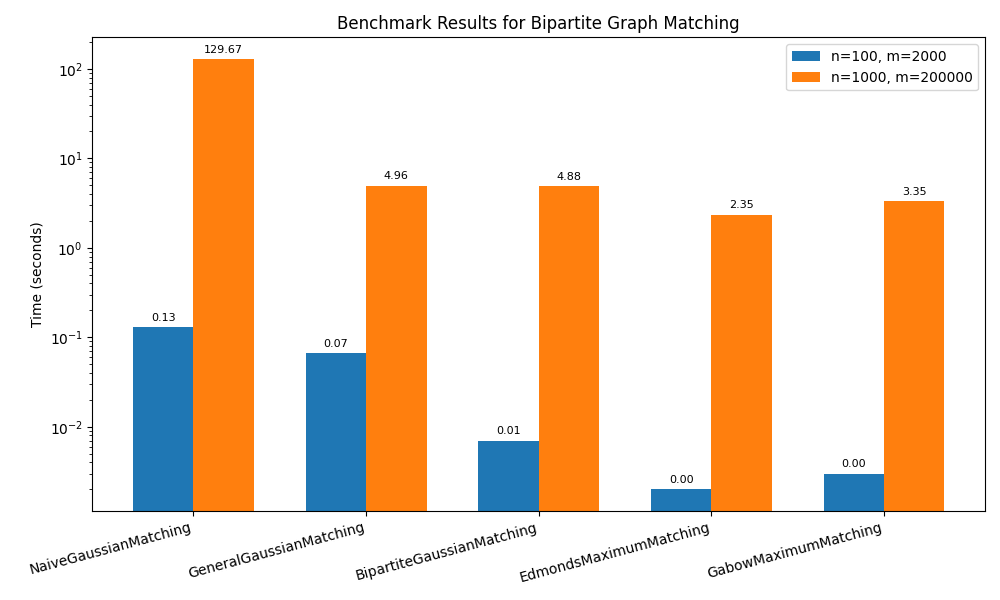
\includegraphics[width=\linewidth]{4_implementation/plots/plot_bp_matching.png}
\end{figure}

\begin{table}[h!]
\centering
\label{tab:benchmark_2}
\begin{tabular}{lccc}
\hline
\textbf{Algorithm} 
& \begin{tabular}[c]{@{}c@{}}$n=100$ \\ $m=2000$\end{tabular}
& \begin{tabular}[c]{@{}c@{}}$n=1000$ \\ $m=200000$\end{tabular} \\
\hline
\textsc{NaiveGaussianMatching} & 150 ms & 147.25 s \\
\textsc{GeneralGaussianMatching} & 23 ms & 11.79 s \\
\hdashline
\textsc{EdmondsMaximumMatching} & 2 ms & 2.44 s \\
\textsc{GabowMaximumMatching} & 3 ms & 3.56 s \\
\hline
\end{tabular}
\caption{Benchmark Results for General Graph Matching}
\end{table}

\begin{figure}[H]
\centering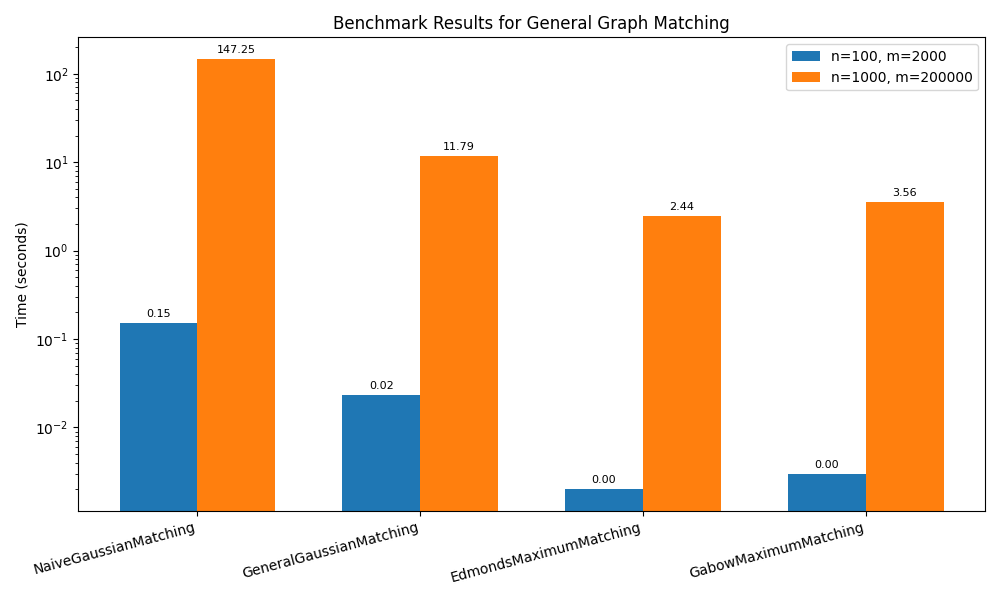
\includegraphics[width=\linewidth]{4_implementation/plots/plot_gen_matching_1.png}
\end{figure}

The implemented \textsc{GeneralGaussianMatching} and \textsc{BipartiteGaussianMatching} algorithms are slower than the compared algorithms. There are some improvements to be made that can improve the running time of both these algorithms. We will discuss them in the later section.

It is also noteworthy that there is a substantial improvement between these algorithms and the \textsc{NaiveGaussianMatching} algorithm running in $O(n^3)$.

We also consider a different benchmark. We present a graph showing how does the \textsc{GeneralGaussianMatching} changes for a different density graphs. Each test case consists of $10$ random graphs with $500$ vertices and varying number of edges $m\in\{1000,5000,10000,50000,100000\}$. As we can see, there is little to no change between the test cases with $m = 5000$ and $m = 100000$. Furthermore, the running time decreases for the largest test. This may be caused by the fact that more edges become allowed in dense graphs. This causes the greedy algorithm to match more vertices, thus reducing the total running time of the algorithm.

\begin{figure}[H]
\centering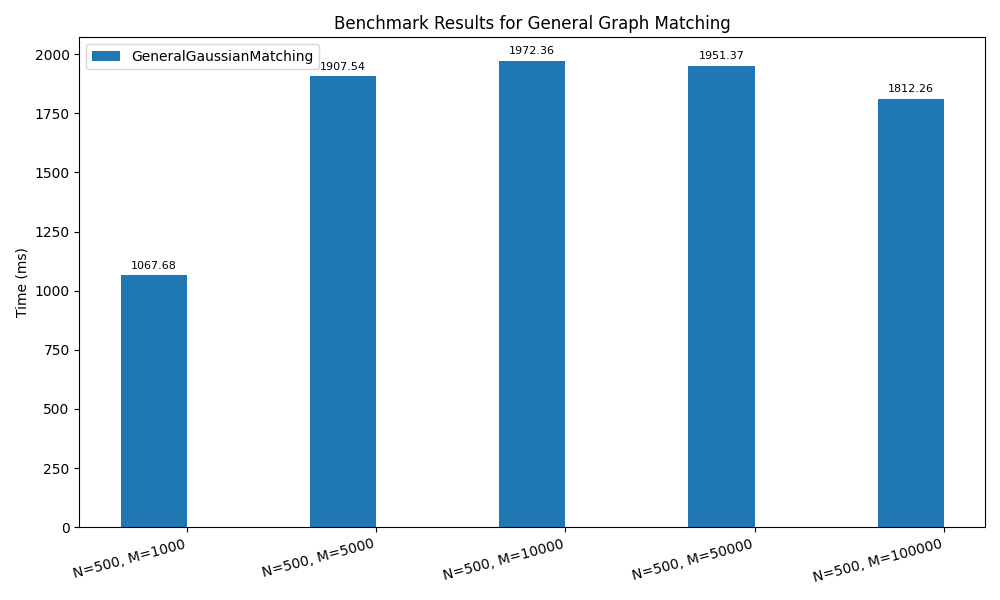
\includegraphics[width=\linewidth]{4_implementation/plots/plot_gen_matching_2.png}
\end{figure}

\subsection{Further work}
There is a number of things that can be further done to improve the above results. Because of the limited time and a great effort put nonetheless, we left a few simplifications in the implementation. Here is a list of improvements that could be made:
\begin{itemize}
    \item Implement fast matrix multiplication and an matrix inverse algorithm, both running in $O(n^\omega)$;
    \item Replace naive implementation of dynamic component with a proper, polylogarithmic one;
    \item Handle separately the largest component in the \textsc{Partition} component.
\end{itemize}

\section{Electrical flow}
\subsection{Implementation details}
While the original paper by Mądry \cite{madry} does only contain a formula driven description of the algorithm, we have developed a pseudocde and a working \texttt{C++} implementation. The main part of the algorithm consists of five files:
\begin{itemize}
    \item \texttt{cpp/ElectricalFlow.cpp}
    \item \texttt{cpp/FlowNetwork.cpp}
    \item \texttt{cpp/ElectricalNetwork.cpp}
    \item \texttt{cpp/NaiveLaplaceSolver.cpp}*
    \item \texttt{cpp/NaiveDynamicTrees.cpp}*
\end{itemize}

We also introduce \textsc{FlowRounding} implementation based on \cite{flow_rounding} that was not include in \cite{madry} explicitly. It utilizes a data structure called \textit{dynamic trees} introduced in \cite{dynamic_trees}. This data structure was implemented in a naive way that does not match the time complexity of \cite{dynamic_trees}. Likewise, the \texttt{NaiveLaplaceSolver} is a simplified implementation using \textit{Moore-Penrose pseudo-inverse}. The \textsc{ElectricalFlow} algorithm can be further improved by providing faster implementations of both \textsc{LaplaceSolver} and \textsc{DynamicTrees}.  

\subsection{Benchmark}
We present a benchmark of the implemented algorithm. We compare its runtime to some algorithms already implemented in \texttt{Koala/NetworKit} and \texttt{NetworKit} itself. We present two test cases based on the size of $n, m$ and $\max w$, each containing $10$ random generated test.

\begin{table}[H]
\centering
\label{tab:benchmark_3}
\begin{tabular}{lccc}
\hline
\textbf{Algorithm} 
& \begin{tabular}[c]{@{}c@{}}$n=100$ \\ $m=2000$ \\ $\max w=5$\end{tabular}
& \begin{tabular}[c]{@{}c@{}}$n=1000$ \\ $m=200000$ \\ $\max w=2$\end{tabular} \\
\hline
\textsc{ElectricalFlow} & 7.28 s & 220 s \\
\textsc{ElectricalFlow w/o rounding} & 7.28 s & 222 s \\
\hdashline
\textsc{BoykovKolmogorovFlow} & 23 ms & 534 ms \\
\textsc{KingRaoTarjanFlow} & 0.53 ms & 4.24 ms \\
\textsc{PushRelabel} & 0.33 ms & 0.77 ms \\
\textsc{EdmondsKarp} & 1.16 ms & 4.49 ms \\
\hline
\end{tabular}
\caption{Benchmark Results for General Graph Matching}
\end{table}

\begin{figure}[H]
\centering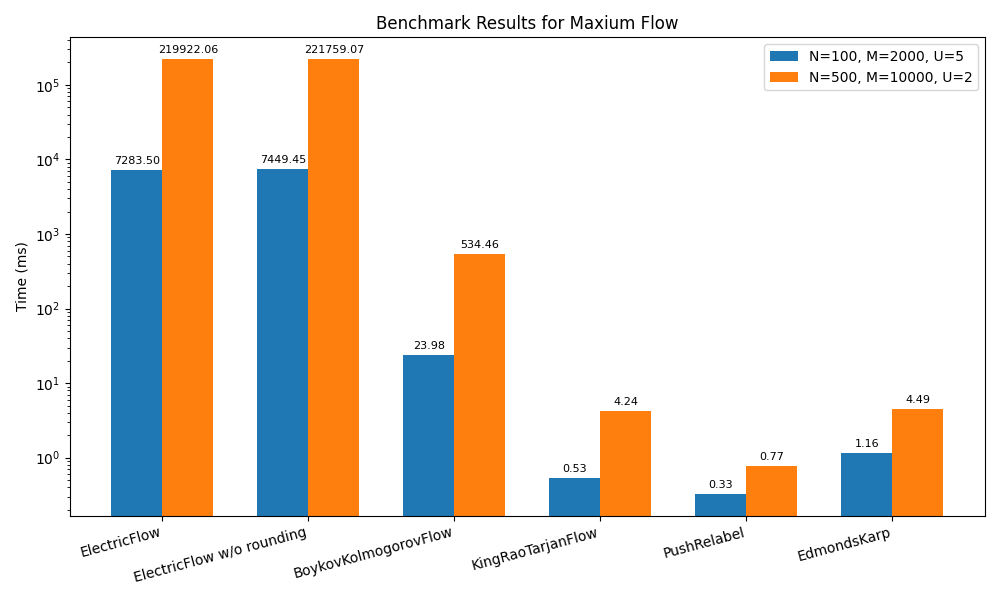
\includegraphics[width=\linewidth]{4_implementation/plots/plot_flow_1.png}
\end{figure}

Unfortunately, the \textsc{ElectricalFlow} algorithm is significantly slower than the other algorithms in the above benchmark. While there some improvements to the current implementation could be made, will not be sufficient to achieve results on par with the compared algorithms. One reason for this issue, is that the algorithm is theory-oriented. While the additional $\log$ in the time complexity might not seem a lot, calling \textsc{RouteFlow} multiple times increased the total runtime more than tenfold.

We present a graph showing the running time difference of \textsc{ElectricalFlow} algorithm for different values of $\max w$. The key difference between those results is the number of times \textsc{RouteFlow} method is called. In the above test cases \textsc{RouteFlow} was called about: $5,6,8,11$ and $15$ times. Based on this fact alone the $\max w=1000$ test case runs about $1.5$ times slower than the $\max w=100$ test. A single \textsc{RuouteFlow} call is slower for the bigger tests as well. For these test cases we got up to $300, 400, 450, 650$ and $800$ iterations per one call. The \textsc{ElectricalFlow} algorithm is thus very sensitive to the weights of the given graph.

\begin{figure}[H]
\centering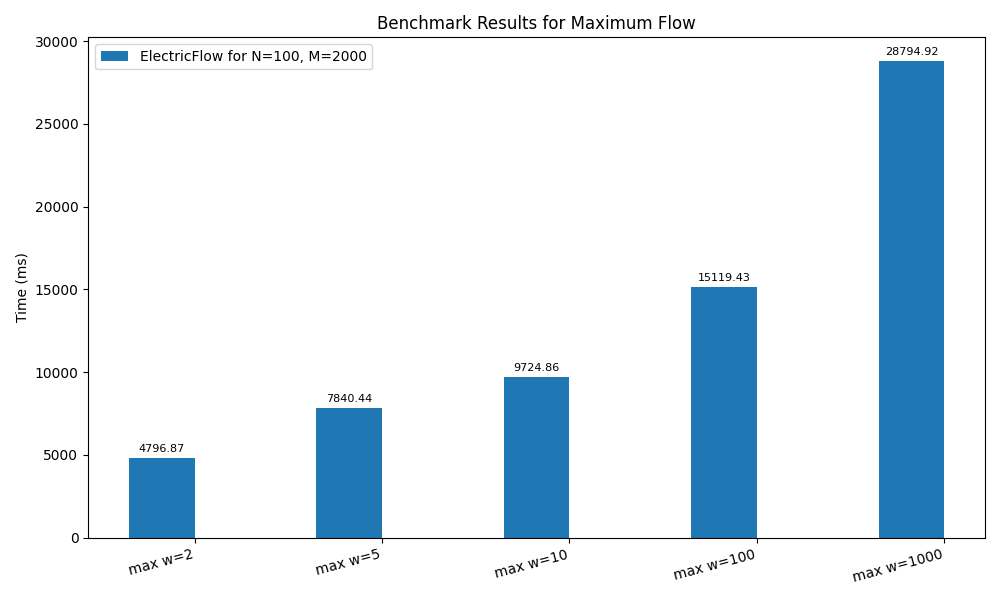
\includegraphics[width=\linewidth]{4_implementation/plots/plot_flow_2.png}
\end{figure}

\subsection{Future work}
Although we succeeded with the implementation of Mądry \cite{madry} maximum flow algorithm, there are some missing futures and improvements that could be added:
\begin{itemize}
    \item Replace Moore-Penrose pseudo-inverse with a faster Laplacian solver;
    \item Add a reduction from directed graphs to the implemented undirected case;
    \item Implement a polylogaritmic dynamic trees data structure for the flow rounding algorithm;
    \item Benchmark algorithm with a preconditioned graph modification.
\end{itemize}
